\documentclass[aspectratio=169,10pt]{beamer}

% Theme & Styling
\usetheme{Madrid}
\usecolortheme{whale}

% -----------------------------------------------------------------------------
% Elegant Obsidian / Dark Aesthetic Palette (Grant Sanderson 3Blue1Brown Style)
% -----------------------------------------------------------------------------
\definecolor{DarkCanvas}{RGB}{12, 16, 24}      % Deep obsidian canvas
\definecolor{DarkBox}{RGB}{20, 27, 40}         % Translucent dark card
\definecolor{DarkBoxInner}{RGB}{26, 36, 54}    % Accent box background
\definecolor{LuminousGold}{RGB}{245, 190, 60}  % Vibrant Gold / ITB Gold
\definecolor{ElectricBlue}{RGB}{80, 165, 250}  % Luminous Sky Blue
\definecolor{TealCyan}{RGB}{45, 212, 191}      % Cyan / Teal
\definecolor{EmeraldGreen}{RGB}{52, 211, 153}  % High-contrast green (Kurva Naik)
\definecolor{CoralRose}{RGB}{251, 113, 133}    % High-contrast rose (Kurva Turun)
\definecolor{PurpleBelok}{RGB}{216, 140, 255}  % Vivid lilac (Titik Belok)
\definecolor{SoftGray}{RGB}{200, 210, 225}     % Readable muted text

% Apply Dark Colors to Beamer Elements
\setbeamercolor{background canvas}{bg=DarkCanvas}
\setbeamercolor{normal text}{fg=white}
\setbeamercolor{structure}{fg=ElectricBlue}
\setbeamercolor{title}{fg=white,bg=DarkBox}
\setbeamercolor{frametitle}{fg=LuminousGold,bg=DarkBox}
\setbeamercolor{footline}{fg=SoftGray!70,bg=DarkCanvas}
\setbeamercolor{headline}{fg=SoftGray!70,bg=DarkCanvas}

% Block Styles in Dark Theme
\setbeamercolor{block title}{fg=white,bg=ElectricBlue!45!black}
\setbeamercolor{block body}{fg=white,bg=DarkBox}
\setbeamercolor{block title example}{fg=white,bg=EmeraldGreen!40!black}
\setbeamercolor{block body example}{fg=white,bg=DarkBox}
\setbeamercolor{block title alerted}{fg=white,bg=CoralRose!45!black}
\setbeamercolor{block body alerted}{fg=white,bg=DarkBox}

% Lists & Numbering
\setbeamercolor{item}{fg=LuminousGold}
\setbeamercolor{subitem}{fg=TealCyan}
\setbeamercolor{enumerate item}{fg=LuminousGold}
\setbeamercolor{enumerate subitem}{fg=TealCyan}

% Packages
\usepackage[utf8]{inputenc}
\usepackage{amsmath,amssymb}
\usepackage{graphicx}
\usepackage{hyperref}
\usepackage{multimedia}
\usepackage{tikz}

\hypersetup{
    colorlinks=true,
    linkcolor=TealCyan,
    urlcolor=ElectricBlue
}

\title[MA1101 Matematika I]{MA1101 Matematika I --- Bab 3: Penggunaan Turunan}
\subtitle{Subtopik 3.2: Kemonotonan dan Kecekungan (\textit{Monotonicity and Concavity})}
\author[FMIPA ITB]{Tim Pengajar MA1101}
\institute[ITB]{Fakultas Matematika dan Ilmu Pengetahuan Alam\\Institut Teknologi Bandung}
\date{Semester 1 Tahun Akademik 2026/2027}

\begin{document}

% -------------------------------------------------------------
% Slide 1: Judul
% -------------------------------------------------------------
\begin{frame}
    \titlepage
\end{frame}

% -------------------------------------------------------------
% Slide 2: Motivasi & Tantangan Sokratik (The Pique)
% -------------------------------------------------------------
\begin{frame}{Tantangan Awal: Membaca Pola Bentuk Kurva}
    \begin{columns}[T]
        \begin{column}{0.55\textwidth}
            \begin{block}{Perilaku Dinamis Kurva $y = f(x)$}
                Saat kita menelusuri kurva dari kiri ke kanan:
                \begin{itemize}
                    \item Kapan kurva \textbf{menanjak} (mendaki) dan kapan \textbf{menurun} (meluncur)?
                    \item Mengapa dua kurva yang sama-sama menanjak bisa memiliki bentuk lengkungan yang sama sekali berbeda?
                \end{itemize}
            \end{block}

            \vspace{0.1cm}
            \begin{alertblock}{Pertanyaan Sokratik}
                Bagaimana membedakan kurva yang melengkung \textit{"menampung air"} versus yang \textit{"menumpahkan air"}?\\
                Informasi apakah yang disimpan oleh \textbf{laju perubahan kemiringan garis singgung}?
            \end{alertblock}
        \end{column}

        \begin{column}{0.42\textwidth}
            \centering
            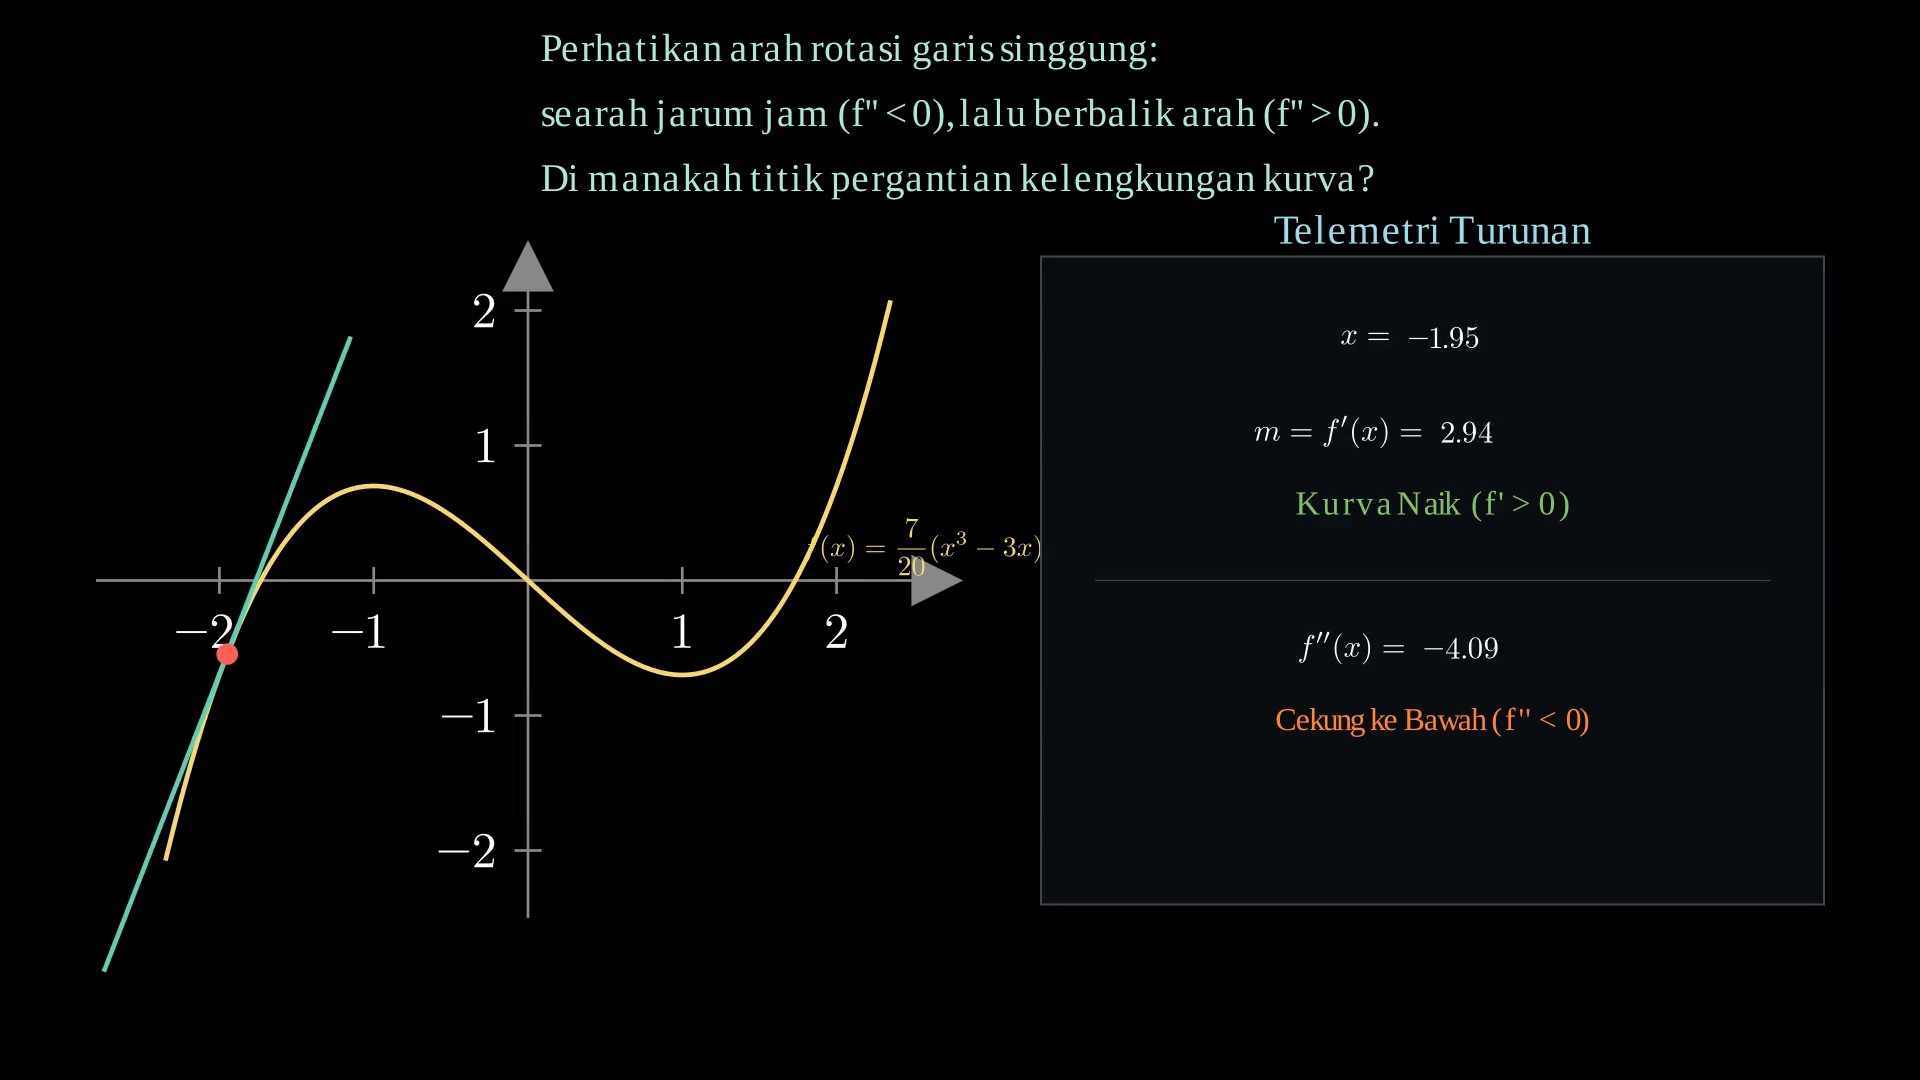
\includegraphics[width=\textwidth]{keyframe_kemonotonan_kecekungan.png}\\
            \vspace{0.1cm}
            {\scriptsize \color{SoftGray} \textit{Telemetri Turunan: Memadukan $f'(x)$ dan $f''(x)$}}
        \end{column}
    \end{columns}
\end{frame}

% -------------------------------------------------------------
% Slide 3: Definisi & Teorema Kemonotonan (Turunan Pertama)
% -------------------------------------------------------------
\begin{frame}{Kemonotonan Fungsi: Arah Gerak Kurva}
    \begin{columns}[T]
        \begin{column}{0.48\textwidth}
            \begin{block}{Definisi Formal Kemonotonan}
                Misalkan $f$ terdefinisi pada selang $I$. Untuk setiap $x_1, x_2 \in I$ dengan $x_1 < x_2$:
                \begin{itemize}
                    \item $f$ \textbf{monoton naik} jika:
                    \[
                        f(x_1) < f(x_2)
                    \]
                    \item $f$ \textbf{monoton turun} jika:
                    \[
                        f(x_1) > f(x_2)
                    \]
                \end{itemize}
                {\scriptsize \color{SoftGray} Nilai fungsi bertambah (naik) atau berkurang (turun) saat melangkah ke kanan.}
            \end{block}
        \end{column}

        \begin{column}{0.48\textwidth}
            \begin{exampleblock}{Teorema Uji Kemonotonan}
                Misalkan $f$ kontinu pada $[a, b]$ dan terdiferensialkan pada $(a, b)$:
                \begin{enumerate}
                    \item Jika $\mathbf{f'(x) > 0}$ untuk semua $x \in (a, b)$, maka $f$ \textbf{monoton naik} pada $[a, b]$.
                    \item Jika $\mathbf{f'(x) < 0}$ untuk semua $x \in (a, b)$, maka $f$ \textbf{monoton turun} pada $[a, b]$.
                \end{enumerate}
            \end{exampleblock}

            \begin{alertblock}{Interpretasi Geometri}
                Kemiringan garis singgung $m = f'(x)$:
                \begin{itemize}
                    \item $m > 0 \implies$ garis condong menanjak ke kanan.
                    \item $m < 0 \implies$ garis condong menurun ke kanan.
                \end{itemize}
            \end{alertblock}
        \end{column}
    \end{columns}
\end{frame}

% -------------------------------------------------------------
% Slide 4: Simulasi Dinamis: Definisi Monoton Naik
% -------------------------------------------------------------
\begin{frame}{Simulasi Dinamis: Definisi Formal Fungsi Monoton Naik}
    \begin{columns}[c]
        \begin{column}{0.62\textwidth}
            \centering
            % Embedded video untuk presenter (Pympress / PDFPC / Okular)
            \movie[width=8.8cm,height=4.95cm,poster,showcontrols=true]{%
                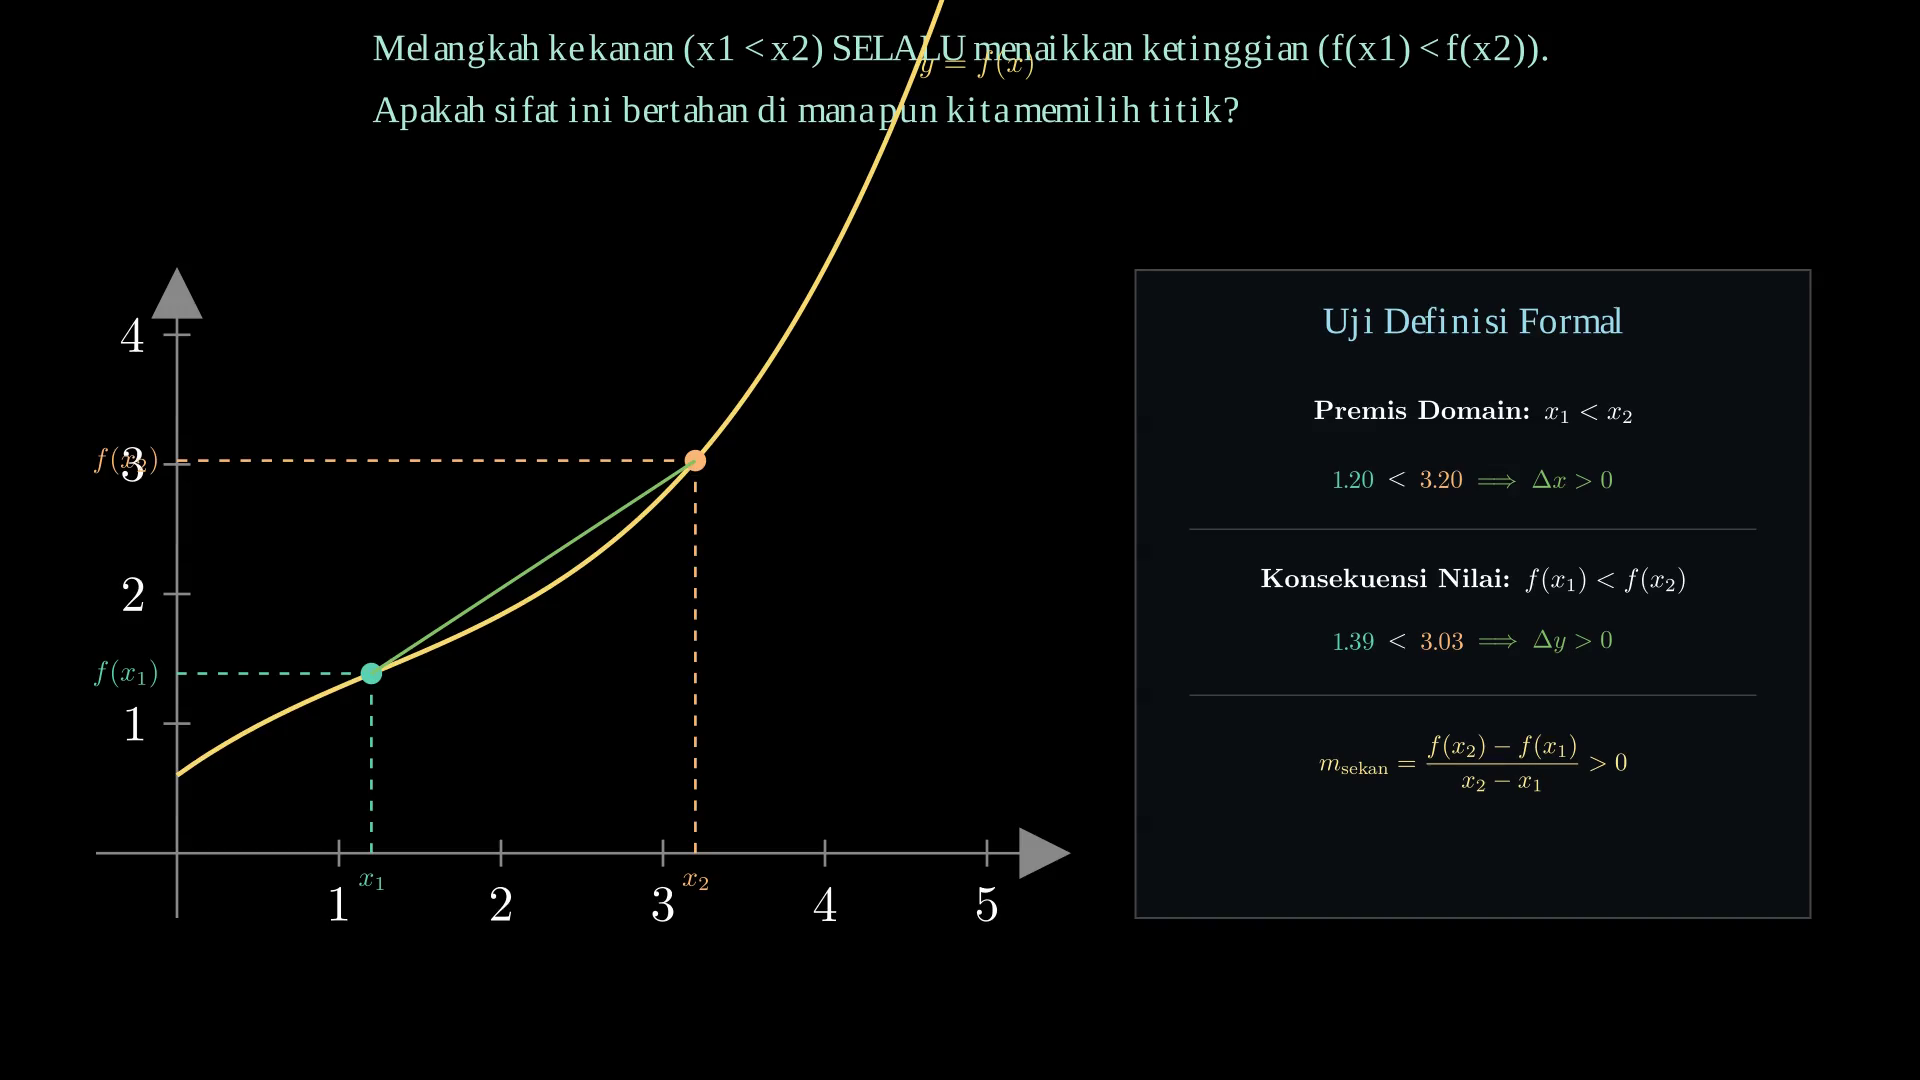
\includegraphics[height=0.55\textheight]{keyframe_monoton_naik.png}%
            }{MonotonicIncreasingScene.ogv}
            
            \vspace{0.15cm}
            \href{file:MonotonicIncreasingScene.mp4}{%
                \beamergotobutton{\normalsize $\blacktriangleright$ Putar Animasi (\texttt{MonotonicIncreasingScene.mp4})}%
            }
        \end{column}

        \begin{column}{0.36\textwidth}
            \begin{block}{Karakteristik Kunci}
                \begin{itemize}
                    \item $\forall x_1 < x_2 \implies f(x_1) < f(x_2)$.
                    \item $\Delta x > 0 \implies \Delta y > 0$.
                    \item Kemiringan sekan selalu positif:
                    \[
                        m_{\text{sekan}} = \frac{\Delta y}{\Delta x} > 0
                    \]
                    \item Menuju konsep turunan:
                    \[
                        f'(x) = \lim_{\Delta x \to 0} \frac{\Delta y}{\Delta x} \ge 0
                    \]
                \end{itemize}
            \end{block}
        \end{column}
    \end{columns}
\end{frame}

% -------------------------------------------------------------
% Slide 4: Definisi & Teorema Kecekungan (Turunan Kedua)
% -------------------------------------------------------------
\begin{frame}{Kecekungan Kurva: Arah Lengkungan (\textit{Concavity})}
    \begin{columns}[T]
        \begin{column}{0.48\textwidth}
            \begin{block}{Definisi Kecekungan via Turunan Pertama}
                Misalkan $f$ terdiferensialkan pada selang buka $I$:
                \begin{itemize}
                    \item $f$ \textbf{cekung ke atas} (\textit{concave up} / $\cup$) jika $f'$ \textbf{naik} pada $I$.\\
                    {\scriptsize $\implies$ Garis singgung berada di \textbf{bawah} kurva.}
                    \item $f$ \textbf{cekung ke bawah} (\textit{concave down} / $\cap$) jika $f'$ \textbf{turun} pada $I$.\\
                    {\scriptsize $\implies$ Garis singgung berada di \textbf{atas} kurva.}
                \end{itemize}
            \end{block}
        \end{column}

        \begin{column}{0.48\textwidth}
            \begin{exampleblock}{Teorema Uji Kecekungan (Turunan Kedua)}
                Misalkan $f$ terdiferensialkan dua kali pada selang buka $I$:
                \begin{enumerate}
                    \item Jika $\mathbf{f''(x) > 0}$ untuk semua $x \in I$, maka $f$ \textbf{cekung ke atas} pada $I$.
                    \item Jika $\mathbf{f''(x) < 0}$ untuk semua $x \in I$, maka $f$ \textbf{cekung ke bawah} pada $I$.
                \end{enumerate}
            \end{exampleblock}

            \begin{alertblock}{Intuisi Rotasi Garis Singgung}
                \begin{itemize}
                    \item $f'' > 0 \implies$ gradien $m$ bertambah (berotasi \textbf{berlawanan} arah jarum jam).
                    \item $f'' < 0 \implies$ gradien $m$ berkurang (berotasi \textbf{searah} jarum jam).
                \end{itemize}
            \end{alertblock}
        \end{column}
    \end{columns}
\end{frame}

% -------------------------------------------------------------
% Slide 5: Simulasi Video Interaktif
% -------------------------------------------------------------
\begin{frame}{Simulasi Dinamis: Pelacakan Gradien, Kemonotonan \& Titik Belok}
    \centering
    % Embedded video untuk presenter (Pympress / PDFPC / Okular)
    \movie[width=9.6cm,height=5.4cm,poster,showcontrols=true]{%
        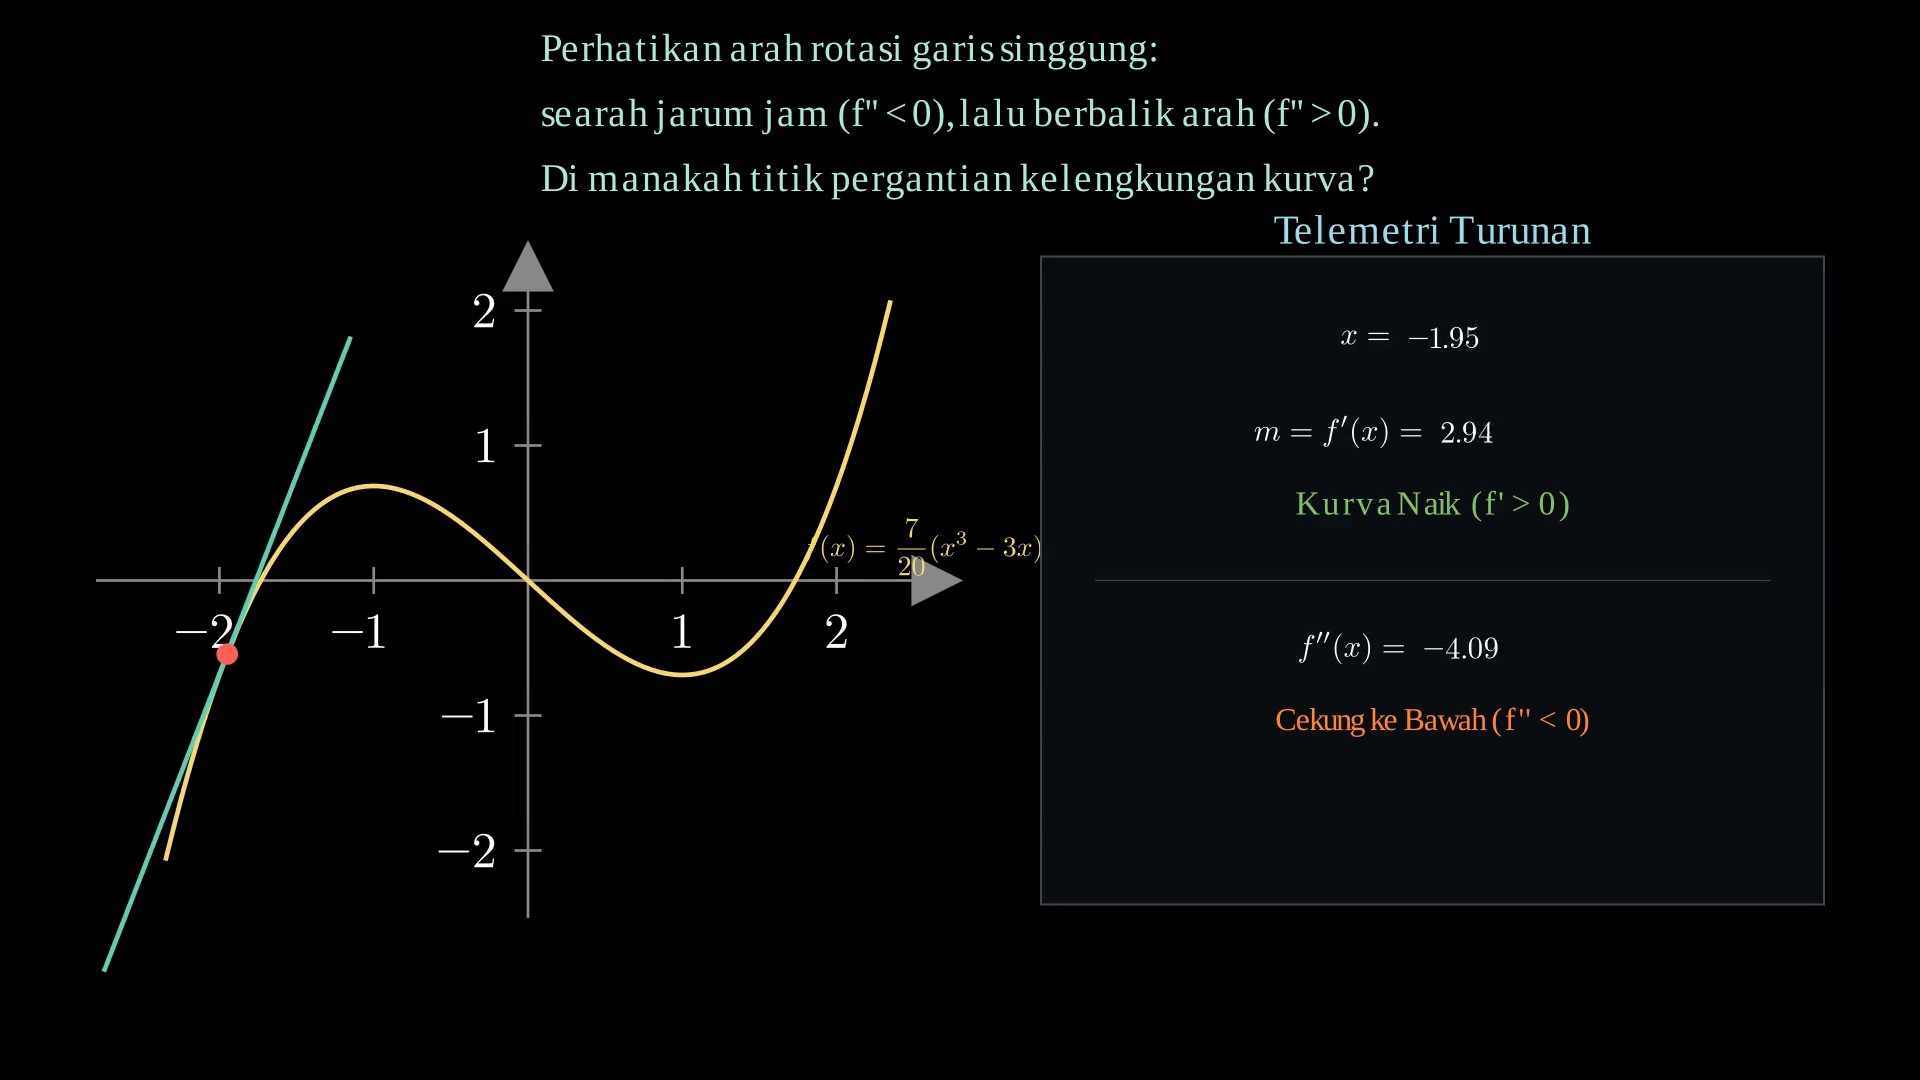
\includegraphics[height=0.55\textheight]{keyframe_kemonotonan_kecekungan.png}%
    }{MonotonicityConcavityScene.ogv}
    
    \vspace{0.2cm}
    \href{file:MonotonicityConcavityScene.mp4}{%
        \beamergotobutton{\normalsize $\blacktriangleright$ Putar Video (\texttt{MonotonicityConcavityScene.mp4})}%
    }
    
    \vspace{0.15cm}
    {\scriptsize \color{SoftGray} \textit{Klik poster untuk pemutaran otomatis di Pympress/Okular, atau klik tombol untuk memutar di MPV/VLC.}}
\end{frame}

% -------------------------------------------------------------
% Slide 6: Titik Belok (Point of Inflection)
% -------------------------------------------------------------
\begin{frame}{Titik Belok (\textit{Point of Inflection})}
    \begin{columns}[T]
        \begin{column}{0.48\textwidth}
            \begin{block}{Definisi Titik Belok}
                Titik $(c, f(c))$ pada kurva kontinu disebut \textbf{Titik Belok} jika:
                \begin{enumerate}
                    \item Terjadi \textbf{perubahan tanda kecekungan} $f''$ di sekitar $x = c$.
                    \item Kurva memiliki \textbf{garis singgung} di titik tersebut.
                \end{enumerate}
                {\scriptsize \color{SoftGray} Garis singgung \textbf{memotong / menembus kurva} di titik belok.}
            \end{block}
        \end{column}

        \begin{column}{0.48\textwidth}
            \begin{exampleblock}{Mencari Calon Titik Belok}
                Titik belok hanya dapat terjadi di titik $c$ di mana:
                \[
                    \mathbf{f''(c) = 0} \quad \text{atau} \quad \mathbf{f''(c) \text{ tidak ada}}
                \]
                {\scriptsize \color{SoftGray} \textbf{Peringatan}: Syarat perlu, bukan cukup (contoh: $f(x)=x^4$).}
            \end{exampleblock}
        \end{column}
    \end{columns}

    \vspace{0.02cm}
    \begin{exampleblock}{Diagram Garis Bilangan: Kriteria Perubahan Tanda $f''(x)$}
        \centering
        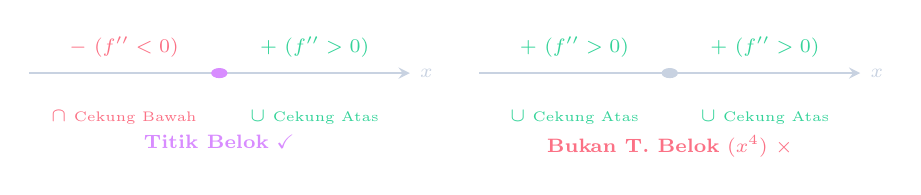
\begin{tikzpicture}[xscale=1.1, yscale=0.65, font=\scriptsize]
            % Kasus A: Perubahan Tanda -> Titik Belok
            \draw[->, >=stealth, thick, SoftGray] (-2.2, 0) -- (2.2, 0) node[right, SoftGray] {$x$};
            \filldraw[PurpleBelok] (0, 0) circle (2.5pt) node[below=2pt, white] {$c$};
            \node[above=2pt, CoralRose] at (-1.1, 0) {$\mathbf{-}\ (f'' < 0)$};
            \node[above=2pt, EmeraldGreen] at (1.1, 0) {$\mathbf{+}\ (f'' > 0)$};
            \node[below=10pt, CoralRose] at (-1.1, 0) {$\cap$ \tiny Cekung Bawah};
            \node[below=10pt, EmeraldGreen] at (1.1, 0) {$\cup$ \tiny Cekung Atas};
            \node[below=19pt, PurpleBelok] at (0, 0) {\textbf{Titik Belok} $\checkmark$};

            % Kasus B: Tidak Ada Perubahan Tanda -> Bukan Titik Belok (Contoh x^4)
            \begin{scope}[shift={(5.2, 0)}]
                \draw[->, >=stealth, thick, SoftGray] (-2.2, 0) -- (2.2, 0) node[right, SoftGray] {$x$};
                \filldraw[SoftGray] (0, 0) circle (2.5pt) node[below=2pt, white] {$0$};
                \node[above=2pt, EmeraldGreen] at (-1.1, 0) {$\mathbf{+}\ (f'' > 0)$};
                \node[above=2pt, EmeraldGreen] at (1.1, 0) {$\mathbf{+}\ (f'' > 0)$};
                \node[below=10pt, EmeraldGreen] at (-1.1, 0) {$\cup$ \tiny Cekung Atas};
                \node[below=10pt, EmeraldGreen] at (1.1, 0) {$\cup$ \tiny Cekung Atas};
                \node[below=19pt, CoralRose] at (0, 0) {\textbf{Bukan T. Belok} ($x^4$) $\times$};
            \end{scope}
        \end{tikzpicture}
    \end{exampleblock}
\end{frame}

% -------------------------------------------------------------
% Slide 7: Uji Turunan Pertama untuk Ekstrem Lokal
% -------------------------------------------------------------
\begin{frame}{Uji Turunan Pertama untuk Ekstrem Relatif}
    \begin{block}{Teorema Uji Turunan Pertama (\textit{First Derivative Test})}
        Misalkan $c$ adalah titik kritis dari fungsi kontinu $f$ pada selang buka yang memuat $c$:
    \end{block}

    \vspace{0.15cm}
    \begin{columns}[T]
        \begin{column}{0.32\textwidth}
            \begin{exampleblock}{1. Maksimum Lokal}
                Tanda $f'$ berubah dari \textbf{positif ke negatif}:
                \[
                    f'(x) > 0 \;\xrightarrow{c}\; f'(x) < 0
                \]
                Kurva mendaki lalu menuruni bukit $\implies f(c)$ adalah \textbf{Maksimum Lokal}.
            \end{exampleblock}
        \end{column}

        \begin{column}{0.32\textwidth}
            \begin{exampleblock}{2. Minimum Lokal}
                Tanda $f'$ berubah dari \textbf{negatif ke positif}:
                \[
                    f'(x) < 0 \;\xrightarrow{c}\; f'(x) > 0
                \]
                Kurva meluncur turun lalu mendaki keluar lembah $\implies f(c)$ adalah \textbf{Minimum Lokal}.
            \end{exampleblock}
        \end{column}

        \begin{column}{0.32\textwidth}
            \begin{alertblock}{3. Bukan Ekstrem}
                Tanda $f'$ \textbf{tidak berubah}:
                \[
                    + \;\to\; + \quad \text{atau} \quad - \;\to\; -
                \]
                Contoh: $f(x) = x^3$ di $x=0$, $f'(x) = 3x^2 \ge 0$ $\implies$ bukan nilai ekstrem!
            \end{alertblock}
        \end{column}
    \end{columns}
\end{frame}

% -------------------------------------------------------------
% Slide 8: Uji Turunan Kedua untuk Ekstrem Lokal
% -------------------------------------------------------------
\begin{frame}{Uji Turunan Kedua untuk Ekstrem Relatif}
    \begin{block}{Teorema Uji Turunan Kedua (\textit{Second Derivative Test})}
        Misalkan $f'$ dan $f''$ kontinu pada selang buka yang memuat titik stasioner $c$ di mana $\mathbf{f'(c) = 0}$:
    \end{block}

    \vspace{0.05cm}
    \begin{columns}[T]
        \begin{column}{0.48\textwidth}
            \begin{alertblock}{1. $\mathbf{f''(c) < 0}$ (Cekung ke Bawah $\cap$)}
                Garis singgung mendatar di puncak mangkok:
                \[
                    f(c) \text{ adalah } \textbf{Maksimum Lokal}
                \]
            \end{alertblock}
        \end{column}

        \begin{column}{0.48\textwidth}
            \begin{exampleblock}{2. $\mathbf{f''(c) > 0}$ (Cekung ke Atas $\cup$)}
                Garis singgung mendatar di dasar mangkok:
                \[
                    f(c) \text{ adalah } \textbf{Minimum Lokal}
                \]
            \end{exampleblock}
        \end{column}
    \end{columns}

    \vspace{0.05cm}
    \begin{block}{Diagram Garis Bilangan Tanda $f'$ di Sekitar Titik Stasioner}
        \centering
        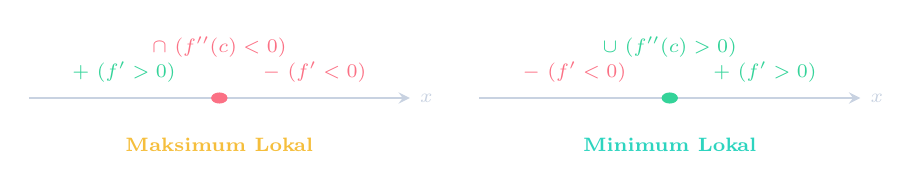
\begin{tikzpicture}[xscale=1.1, yscale=0.72, font=\scriptsize]
            % Kasus 1: f''(c) < 0 -> Maks Lokal (+ ke -)
            \draw[->, >=stealth, thick, SoftGray] (-2.2, 0) -- (2.2, 0) node[right, SoftGray] {$x$};
            \filldraw[CoralRose] (0, 0) circle (2.5pt) node[below=2pt, white] {$c$};
            \node[above=2pt, EmeraldGreen] at (-1.1, 0) {$\mathbf{+}\ (f' > 0)$};
            \node[above=2pt, CoralRose] at (1.1, 0) {$\mathbf{-}\ (f' < 0)$};
            \node[above=11pt, CoralRose] at (0, 0) {$\cap\ (f''(c) < 0)$};
            \node[below=11pt, LuminousGold] at (0, 0) {\textbf{Maksimum Lokal}};

            % Kasus 2: f''(c) > 0 -> Min Lokal (- ke +)
            \begin{scope}[shift={(5.2, 0)}]
                \draw[->, >=stealth, thick, SoftGray] (-2.2, 0) -- (2.2, 0) node[right, SoftGray] {$x$};
                \filldraw[EmeraldGreen] (0, 0) circle (2.5pt) node[below=2pt, white] {$c$};
                \node[above=2pt, CoralRose] at (-1.1, 0) {$\mathbf{-}\ (f' < 0)$};
                \node[above=2pt, EmeraldGreen] at (1.1, 0) {$\mathbf{+}\ (f' > 0)$};
                \node[above=11pt, EmeraldGreen] at (0, 0) {$\cup\ (f''(c) > 0)$};
                \node[below=11pt, TealCyan] at (0, 0) {\textbf{Minimum Lokal}};
            \end{scope}
        \end{tikzpicture}
    \end{block}
    \centering
    {\scriptsize \color{SoftGray} \textit{Catatan: Jika $f''(c) = 0$, uji ini inkonklusif (gunakan Uji Turunan Pertama).}}
\end{frame}

% -------------------------------------------------------------
% Slide 9: Contoh Soal Komprehensif
% -------------------------------------------------------------
\begin{frame}{Contoh Soal Komprehensif: Polinomial Orde 3}
    \textbf{Soal}: Analisis kemonotonan, kecekungan, ekstrem lokal, dan titik belok dari $f(x) = 2x^3 - 3x^2 - 12x + 5$.

    \pause
    \vspace{0.1cm}
    \begin{columns}[T]
        \begin{column}{0.48\textwidth}
            \begin{block}{Langkah 1: Analisis Kemonotonan ($f'$)}
                \[
                    f'(x) = 6x^2 - 6x - 12 = 6(x - 2)(x + 1)
                \]
                Titik kritis: $x = -1$ dan $x = 2$.
                \begin{itemize}
                    \item $x \in (-\infty, -1) \implies f' > 0$ (\textbf{Naik})
                    \item $x \in (-1, 2) \implies f' < 0$ (\textbf{Turun})
                    \item $x \in (2, \infty) \implies f' > 0$ (\textbf{Naik})
                \end{itemize}
                $\implies$ \textbf{Maks Lokal}: $f(-1) = 12$\\
                $\implies$ \textbf{Min Lokal}: $f(2) = -15$
            \end{block}
        \end{column}

        \begin{column}{0.48\textwidth}
            \begin{exampleblock}{Langkah 2: Analisis Kecekungan ($f''$)}
                \[
                    f''(x) = 12x - 6 = 6(2x - 1)
                \]
                Pembuat nol turunan kedua: $x = 1/2$.
                \begin{itemize}
                    \item $x \in (-\infty, 1/2) \implies f'' < 0$ (\textbf{Cekung ke Bawah})
                    \item $x \in (1/2, \infty) \implies f'' > 0$ (\textbf{Cekung ke Atas})
                \end{itemize}
                Perubahan kecekungan terjadi di $x = 1/2$.
                \[
                    f(1/2) = 2(1/8) - 3(1/4) - 12(1/2) + 5 = -3/2
                \]
                $\implies$ \textbf{Titik Belok}: $\left(\frac{1}{2}, -\frac{3}{2}\right)$
            \end{exampleblock}
        \end{column}
    \end{columns}
\end{frame}

% -------------------------------------------------------------
% Slide 10: Diagram Garis Bilangan Bertumpuk
% -------------------------------------------------------------
\begin{frame}{Diagram Garis Bilangan Bertumpuk: Rekonstruksi Kurva}
    \begin{block}{Analisis Gabungan Tanda $f'(x)$ dan $f''(x)$ untuk $f(x) = 2x^3 - 3x^2 - 12x + 5$}
        Garis bilangan bertumpuk memadukan arah gerak (naik/turun) dan bentuk kecekungan ($\cap$ / $\cup$):
    \end{block}

    \vspace{0.1cm}
    \centering
    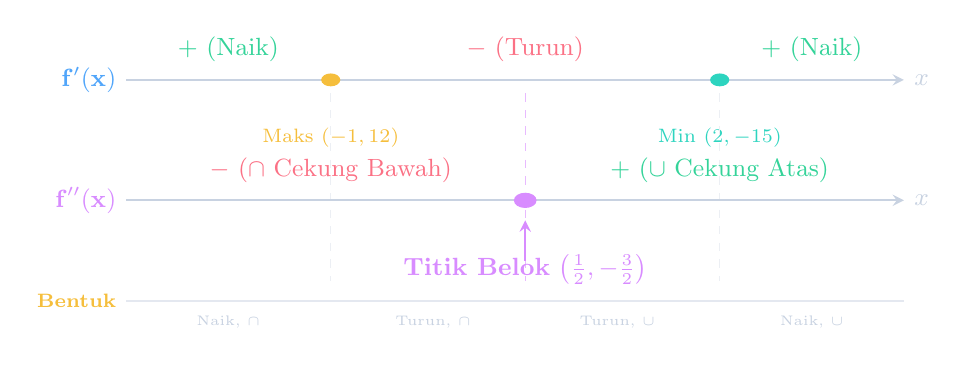
\begin{tikzpicture}[xscale=1.3, yscale=0.85, font=\small]
        % Garis 1: Tanda f'(x)
        \draw[->, >=stealth, thick, SoftGray] (-3.8, 1.2) -- (3.8, 1.2) node[right, SoftGray] {$x$};
        \node[left, ElectricBlue] at (-3.8, 1.2) {$\mathbf{f'(x)}$};
        
        \filldraw[LuminousGold] (-1.8, 1.2) circle (2.5pt) node[below=3pt, white] {$\mathbf{-1}$};
        \filldraw[TealCyan] (2.0, 1.2) circle (2.5pt) node[below=3pt, white] {$\mathbf{2}$};
        
        \node[above=3pt, EmeraldGreen] at (-2.8, 1.2) {$\mathbf{+}\ \text{(Naik)}$};
        \node[above=3pt, CoralRose] at (0.1, 1.2) {$\mathbf{-}\ \text{(Turun)}$};
        \node[above=3pt, EmeraldGreen] at (2.9, 1.2) {$\mathbf{+}\ \text{(Naik)}$};
        
        \node[below=14pt, LuminousGold] at (-1.8, 1.2) {\scriptsize Maks $(-1, 12)$};
        \node[below=14pt, TealCyan] at (2.0, 1.2) {\scriptsize Min $(2, -15)$};

        % Garis Pandu Vertikal
        \draw[dashed, SoftGray!35] (-1.8, 1.0) -- (-1.8, -1.8);
        \draw[dashed, PurpleBelok!60] (0.1, 1.0) -- (0.1, -1.8);
        \draw[dashed, SoftGray!35] (2.0, 1.0) -- (2.0, -1.8);

        % Garis 2: Tanda f''(x)
        \draw[->, >=stealth, thick, SoftGray] (-3.8, -0.6) -- (3.8, -0.6) node[right, SoftGray] {$x$};
        \node[left, PurpleBelok] at (-3.8, -0.6) {$\mathbf{f''(x)}$};
        
        \filldraw[PurpleBelok] (0.1, -0.6) circle (3pt) node[below=3pt, white] {$\mathbf{\frac{1}{2}}$};
        \node[above=3pt, CoralRose] at (-1.8, -0.6) {$\mathbf{-}\ (\cap\ \text{Cekung Bawah})$};
        \node[above=3pt, EmeraldGreen] at (2.0, -0.6) {$\mathbf{+}\ (\cup\ \text{Cekung Atas})$};
        
        \node[below=16pt, PurpleBelok] at (0.1, -0.6) {\textbf{Titik Belok} $\left(\frac{1}{2}, -\frac{3}{2}\right)$};
        \draw[->, >=stealth, PurpleBelok, thick] (0.1, -1.5) -- (0.1, -0.9);

        % Garis Sintesis Bentuk
        \node[left, LuminousGold] at (-3.8, -2.1) {\scriptsize \textbf{Bentuk}};
        \draw[thick, SoftGray!50] (-3.8, -2.1) -- (3.8, -2.1);
        \node[below=2pt, SoftGray] at (-2.8, -2.1) {\tiny Naik, $\cap$};
        \node[below=2pt, SoftGray] at (-0.8, -2.1) {\tiny Turun, $\cap$};
        \node[below=2pt, SoftGray] at (1.0, -2.1) {\tiny Turun, $\cup$};
        \node[below=2pt, SoftGray] at (2.9, -2.1) {\tiny Naik, $\cup$};
    \end{tikzpicture}
\end{frame}

% -------------------------------------------------------------
% Slide 10: Contoh Khusus & Jebakan Konseptual
% -------------------------------------------------------------
\begin{frame}{Jebakan Konseptual: Titik Singular \& Garis Singgung Vertikal}
    \begin{columns}[T]
        \begin{column}{0.48\textwidth}
            \begin{alertblock}{Studi Kasus: $f(x) = x^{1/3}$ (Akar Tiga)}
                Perhatikan fungsi $f(x) = x^{1/3}$ pada $\mathbb{R}$:
                \[
                    f'(x) = \frac{1}{3}x^{-2/3} = \frac{1}{3\sqrt[3]{x^2}}
                \]
                \begin{itemize}
                    \item Untuk semua $x \neq 0$, $x^2 > 0 \implies f'(x) > 0$.
                    \item Kurva \textbf{selalu monoton naik} di seluruh $\mathbb{R}$.
                    \item Di $x = 0$, $f'(0)$ tidak ada (garis singgung vertikal tegak lurus sumbu-$x$).
                \end{itemize}
            \end{alertblock}
        \end{column}

        \begin{column}{0.48\textwidth}
            \begin{exampleblock}{Kecekungan $f(x) = x^{1/3}$}
                Turunan kedua:
                \[
                    f''(x) = -\frac{2}{9}x^{-5/3} = -\frac{2}{9\sqrt[3]{x^5}}
                \]
                \begin{itemize}
                    \item Untuk $x < 0 \implies x^5 < 0 \implies \mathbf{f''(x) > 0}$ (\textbf{Cekung ke Atas}).
                    \item Untuk $x > 0 \implies x^5 > 0 \implies \mathbf{f''(x) < 0}$ (\textbf{Cekung ke Bawah}).
                \end{itemize}
                \textbf{Kesimpulan}: Titik $(0, 0)$ adalah \textbf{Titik Belok}!\\
                {\scriptsize \textit{Meskipun $f''(0)$ tidak ada, kecekungan tetap berbalik arah dan terdapat garis singgung vertikal!}}
            \end{exampleblock}
        \end{column}
    \end{columns}
\end{frame}

% -------------------------------------------------------------
% Slide 11: Latihan Mandiri & Rangkuman
% -------------------------------------------------------------
\begin{frame}{Latihan Mandiri \& Rangkuman Subtopik 3.2}
    \begin{columns}[T]
        \begin{column}{0.48\textwidth}
            \begin{block}{Latihan Mandiri}
                \begin{enumerate}
                    \item Tentukan selang naik/turun, kecekungan, serta titik belok dari fungsi rasional:
                    \[
                        g(x) = \frac{x^2}{x^2 + 3}
                    \]
                    \item Diberikan grafik $y = f'(x)$ berupa parabola terbuka ke atas dengan akar di $x = -2$ dan $x = 3$. Tentukan di mana grafik fungsi asal $f(x)$ cekung ke atas!
                \end{enumerate}
            \end{block}
        \end{column}

        \begin{column}{0.48\textwidth}
            \begin{exampleblock}{Tabel Rangkuman Turunan}
                \centering
                \small
                \setlength{\tabcolsep}{3pt}
                \begin{tabular}{|c|c|c|}
                    \hline
                    \textbf{Tanda} & $\mathbf{f'(x)}$ & $\mathbf{f''(x)}$ \\
                    \hline
                    Positif ($>0$) & Kurva Naik & Cekung ke Atas ($\cup$) \\
                    Negatif ($<0$) & Kurva Turun & Cekung ke Bawah ($\cap$) \\
                    Nol ($=0$) & Titik Stasioner & Calon Titik Belok \\
                    \hline
                \end{tabular}
            \end{exampleblock}

            \vspace{0.15cm}
            \centering
            {\small \textbf{Selamat Belajar \& Sukses Perkuliahan MA1101!}}\\
            {\scriptsize \color{SoftGray} Tim Dosen Matematika I --- FMIPA Institut Teknologi Bandung}
        \end{column}
    \end{columns}
\end{frame}

\end{document}
